% Auto-generated supplement snippet for accuracy-tolerance sensitivity
\subsection{Accuracy-Tolerance Sensitivity}

Table~\ref{tab:epsilon_thresholds} summarizes the trust-activation threshold $\hat{\gamma}$ as a function of the accuracy tolerance $\varepsilon$. The empirical threshold is the smallest sweep-grid $\gamma$ at which the day-51 flow-weighted guidance error exceeds $\varepsilon$. The predicted threshold uses $\hat{\gamma} \approx \varepsilon / D$, where $D$ is estimated from the day-51 error at the smallest sweep $\gamma$ ($D \approx e(d{=}51)/\gamma$).

\begin{table}[!t]
\centering
\caption{Trust-activation threshold $\hat{\gamma}$ versus accuracy tolerance $\varepsilon$, with post-threshold attenuation TIA at $\gamma=0.7$.}
\label{tab:epsilon_thresholds}
\begin{tabular}{lcccc}
\hline
$\varepsilon$ (h) & $\varepsilon$ (min) & $\hat{\gamma}_{\text{emp}}$ & $\hat{\gamma}_{\text{pred}}$ & TIA at $\gamma{=}0.7$ \\
\hline
0.05 & 3.0 & 0.500 & 0.336 & 0.910 \\
0.10 & 6.0 & 0.700 & 0.672 & 0.910 \\
0.15 & 9.0 & --$^{\dagger}$ & 1.007 & 0.746 \\
\hline
\end{tabular}\\[2pt]
\footnotesize{$^{\dagger}$ The day-51 guidance error at $\gamma=1$ is $536$ s, which is just below $\varepsilon = 540$ s, so the empirical threshold lies outside the coarse sweep grid; the analytical prediction places it at $\hat{\gamma} \approx 1.007$.}
\end{table}

\begin{figure}[!t]
\centering
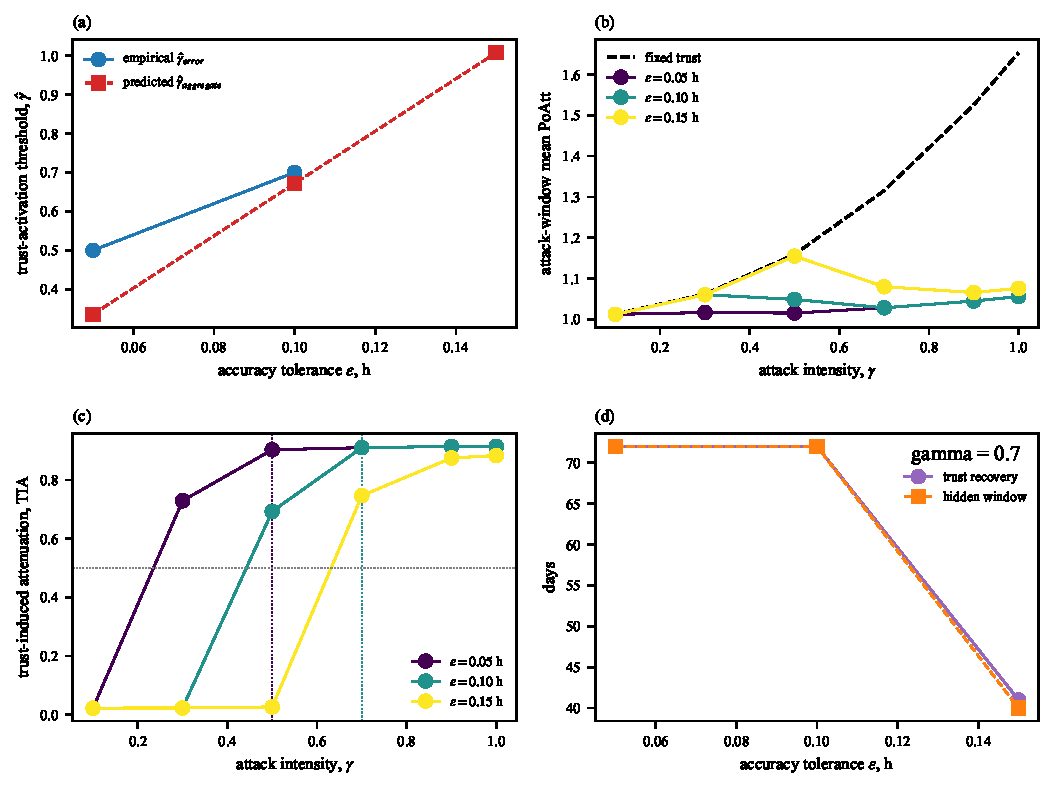
\includegraphics[width=\columnwidth]{fig_epsilon_sensitivity.pdf}
\caption{Accuracy-tolerance sensitivity. (a) Empirical and predicted trust-activation threshold $\hat{\gamma}$ as $\varepsilon$ varies. (b) Attack-window mean PoAtt against $\gamma$ for the fixed-trust baseline and each $\varepsilon$. (c) TIA against $\gamma$, with $\hat{\gamma}$ positions marked. (d) Trust recovery time and hidden vulnerability window against $\varepsilon$.}
\label{fig:epsilon_sensitivity}
\end{figure}

Changing $\varepsilon$ shifts the trust-activation threshold but does not remove the two-regime structure. Smaller $\varepsilon$ values activate trust erosion at lower attack intensities, while larger $\varepsilon$ values expand the stealthy regime. Once the attack intensity exceeds the corresponding threshold, dynamic trust again produces strong attenuation.
